%! Author = Len Washington III
%! Date = 2/3/24

% Preamble
\documentclass[assignment={3},
	duedate={Sunday, March 31, 2024, 11:59 PM CST},
	points={80},
	type={Written},
	template=true
]{cs581homework}

% Packages
\newcommand{\justify}{\textbf{\underline{Justify your answer.}}}

% Document
\begin{document}

\maketitle

\begin{objectives}
	\begin{enumerate}
		\item (10 points) Demonstrate your understanding of Particle Swarm Optimization.
		\item (15 points) Demonstrate your understanding of basic probability rules.
		\item (15 points) Demonstrate your understanding of Bayes Networks.
		\item (25 points) Demonstrate your understanding of Decision Networks.
		\item (15 points) Demonstrate your understanding of Hidden Markov Models.
	\end{enumerate}
\end{objectives}

\problem{10}
Consider the Particle Swarm Optimization problem with the following parameters:\\
$N$ -- number of particles: 5,
$w$ -- inertia weight: 0.3,
$c_{1}$ -- cognitive constant: 1,
$c_{2}$ -- social constant: 1\\

At some time $t$ particles are defined with (assume that this is a maximizing problem):
\begin{table}[H]
	\centering
	\label{tab:problem-1}
	\begin{tabular}{|c|*{2}{P{0.15\textwidth}|}P{0.27\textwidth}|*{3}{c|}}
		\hline
		\textbf{Particle} & \textbf{Position $X_{it}$} & \textbf{Velocity $V_{it}$} & \textbf{Particle’s best $X_{i,best}$} & \textbf{Fitness} & $\mathbf{a}$ & $\mathbf{b}$ \\
		\hline
		1 & [0.2,0.1,0.2] & [0.2,0.1,0.1] & [0.5,0.5,0.1] & 1.0 & 0.10 & 0.23 \\
		\hline
		2 & [0.9,1.1,0.2] & [0.1,0.1,0.0] & [0.2,0.2,0.1] & 0.9 & 0.55 & 0.45 \\
		\hline
		3 & [0.6,1.1,0.6] & [0.0,1.5,0.6] & [0.0,0.0,0.0] & 0.8 & 0.12 & 0.78 \\
		\hline
		4 & [1.2,4.1,1.2] & [0.2,1.1,0.4] & [0.5,0.5,0.1] & 1.2 & 0.89 & 0.54 \\
		\hline
		5 & [1.0,1.0,1.0] & [0.0,0.7,1.0] & [0.3,0.5,0.1] & 0.7 & 0.56 & 0.67 \\
		\hline
	\end{tabular}
\end{table}

What are particle positions at time $t+1$ assuming that $a$ and $b$ are random numbers for cognitive and social influence respectively?

\begin{answerbox}

\end{answerbox}

\problem{15}
Consider the following full joint probability distribution for three Boolean variables $X$, $Y$, and $Z$ \textbf{[show all your work, formulas, etc.]}:\\

\begin{minipage}[t]{0.35\textwidth}
	\begin{table}[H]
		\centering
		\label{tab:prb-2}
		\begin{tabular}{|*{4}{c|}}
			\hline
			$\mathbf{X}$ & $\mathbf{Y}$ & $\mathbf{Z}$ & $\mathbf{P(X,Y,Z)}$\\
			\hline
			T & T & T & 0.03\\
			\hline
			T & T & F & 0.12\\
			\hline
			T & F & T & 0.17\\
			\hline
			T & F & F & 0.18\\
			\hline
			F & T & T & 0.03\\
			\hline
			F & T & F & 0.12\\
			\hline
			F & F & T & 0.24\\
			\hline
			F & F & F & 0.11\\
			\hline
		\end{tabular}
	\end{table}
\end{minipage}\hfill%
\begin{minipage}[t]{0.6\textwidth}
	Calculate probabilities (\textbf{round to 3 decimal places}):
	\begin{enumerate}[label=\alph*) \textbf{[1 pt]}]
		\item P($X$ = F) = \_\_\_\_\_\_\_\_\_\_\_\_\_
		\item P($X$ = T) = \_\_\_\_\_\_\_\_\_\_\_\_\_
		\item P($X$ = T, $Z$ = T) = \_\_\_\_\_\_\_\_\_\_\_\_\_
		\item P($X$ = T $|$ $Y$ = T) = \_\_\_\_\_\_\_\_\_\_\_\_\_
		\item P($Z$ = F $|$ $Y$ = T) = \_\_\_\_\_\_\_\_\_\_\_\_\_
	\end{enumerate}
\end{minipage}

\noindent Answer \textbf{[YES/NO]} the following questions:
\begin{enumerate}[label=\alph*) \textbf{[2.5 pt]},start=6]
	\item Are $X$ and $Y$ independent of each other? \justify
	\begin{answerbox}
	\end{answerbox}
	\item Are $Y$ and $Z$ independent of each other? \justify
	\begin{answerbox}
	\end{answerbox}
	\item Are $Y$ and $Z$ conditionally independent given $X$? \justify
	\begin{answerbox}
	\end{answerbox}
	\item Are $X$ and $Z$ conditionally independent given $Y$? \justify
	\begin{answerbox}
	\end{answerbox}
\end{enumerate}

\problem{15}
Given the following Bayes Network:
\begin{figure}[H]
	\centering
	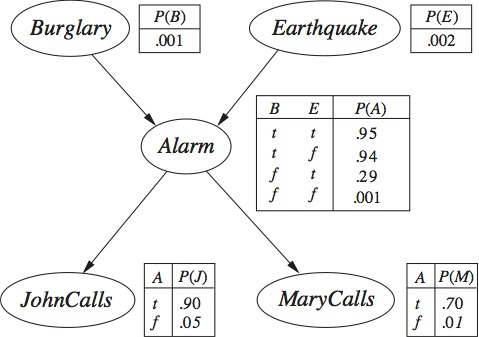
\includegraphics[width=\textwidth]{bayes}
	\label{fig:bayes}
\end{figure}
Use the \textbf{General Inference Procedure} to calculate the probability (\textbf{show all your work}):
\begin{center} P(Alarm = False $|$ Earthquake = True, MaryCalls = False) \end{center}
\begin{answerbox}
\end{answerbox}

\problem{25}
Consider the following decision network (\textbf{note three decisions for D: x, y, z}):
\begin{figure}[H]
	\centering
	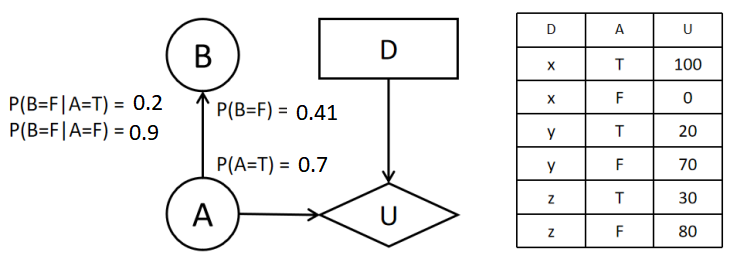
\includegraphics[width=\textwidth]{decision}
	\label{fig:decision}
\end{figure}

\begin{table}[H]
	\centering
	\begin{tabular}{|p{\textwidth}|}
		\hline
		\textbf{A) Complete conditional probability tables for each chance node. [1 pt]:}\\
		\hline
		\iftemplate
		\vspace*{1in}~\\
		\else
		\fi
		\hline
	\end{tabular}
\end{table}

\begin{table}[H]
	\centering
	\begin{tabular}{|p{\textwidth}|}
		\hline
		\textbf{B) Which decision (x, y or z) is best given evidence B = T? Justify your answer. [12 pts]:}\\
		\hline
		\iftemplate
		\vspace*{1in}~\\
		\else
		\fi
		\hline
	\end{tabular}
\end{table}

\begin{table}[H]
	\centering
	\begin{tabular}{|p{\textwidth}|}
		\hline
		\textbf{C) What is the value of information for B? Justify your answer. [12 pts]:}\\
		\hline
		\iftemplate
		\vspace*{1in}~\\
		\else
		\fi
		\hline
	\end{tabular}
\end{table}

\problem{15}
Consider the following Hidden Markov Model (no start/end state - that's fine):

\begin{minipage}[b]{0.45\textwidth}
	\begin{table}[H]
		\centering
		\caption{Transition Probability Matrix}
		\label{tab:transitions}
		\begin{tabular}{|*{6}{c|}}
			\hline
			\textbf{State} & $S_{1}$ & $S_{2}$ & $S_{3}$ & $S_{4}$ & $S_{5}$ \\
			\hline
			$S_{1}$ & 0.02 & 0.70 & 0.11 & 0.08 & 0.09 \\
			\hline
			$S_{2}$ & 0.01 & 0.20 & 0.30 & 0.45 & 0.04 \\
			\hline
			$S_{3}$ & 0.10 & 0.14 & 0.16 & 0.29 & 0.31 \\
			\hline
			$S_{4}$ & 0.80 & 0.03 & 0.04 & 0.01 & 0.12 \\
			\hline
			$S_{5}$ & 0.21 & 0.22 & 0.23 & 0.19 & 0.15 \\
			\hline
		\end{tabular}
	\end{table}
\end{minipage}
\begin{minipage}[b]{0.55\textwidth}
	\begin{table}[H]
		\centering
		\caption{Emission Probability Matrix \textbf{[selected observations only]}}
		\label{tab:emissions}
		\begin{tabular}{|*{6}{c|}}
			\hline
			\textbf{State} & $o_{1}$ & $o_{5}$ & $o_{8}$ & $o_{11}$ & $o_{15}$ \\
			\hline
			$S_{1}$ & 0.10 & 0.04 & 0.05 & 0.11 & 0.21 \\
			\hline
			$S_{2}$ & 0.20 & 0.00 & 0.14 & 0.02 & 0.50 \\
			\hline
			$S_{3}$ & 0.21 & 0.03 & 0.07 & 0.16 & 0.22 \\
			\hline
			$S_{4}$ & 0.83 & 0.08 & 0.06 & 0.00 & 0.00 \\
			\hline
			$S_{5}$ & 0.31 & 0.32 & 0.19 & 0.13 & 0.00 \\
			\hline
		\end{tabular}
	\end{table}
\end{minipage}\\

Given the sequence of observations (in that order): $o_{8}$, $o_{11}$, $o_{5}$, what is the most likely sequence of states that generated it (\textbf{show all your work: formulas and calculations}):

\begin{enumerate}[label=\alph*)]
	\item $S_{1}$, $S_{4}$, $S_{5}$
	\item $S_{2}$, $S_{4}$, $S_{5}$
	\item $S_{1}$, $S_{2}$, $S_{3}$
\end{enumerate}

\end{document}